% SynAthlete-AIoT: final paper draft to the faculty's format (single column, Times 12 pt,
% line spacing 1.25, at least 8 pages, architecture diagram, graphs, 20+ ScienceDirect / IEEE
% Transactions references). Every number comes from generated/*.tex, written by
% `python tasks.py paper-figures` from the experiments/**/metrics.json files (AGENTS.md
% invariant 1). Do not type numbers by hand. Upload to Overleaf: this file, refs_final.bib,
% generated/ and figures/.
\documentclass[12pt,a4paper]{article}
\usepackage[T1]{fontenc}
\usepackage[utf8]{inputenc}
\usepackage{newtxtext,newtxmath}
\usepackage[margin=1in]{geometry}
\usepackage{setspace}
\setstretch{1.25}
\usepackage{graphicx}
\usepackage{booktabs}
\usepackage{xspace}
\usepackage{amsmath}
\usepackage{caption}
\captionsetup{font=small,labelfont=bf,labelsep=period}
\usepackage[numbers,sort&compress]{natbib}
\usepackage[hidelinks]{hyperref}
\graphicspath{{figures/}}
% generated by src/paper/figures.py: do not edit
\newcommand{\canaryAuc}{0.498 (day) and 0.513 (week)\xspace}
\newcommand{\explainSummary}{Explanation checks: n/a.\xspace}
\newcommand{\fusedAuc}{n/a\xspace}
\newcommand{\fusedPrAuc}{n/a\xspace}
\newcommand{\injuryAucRange}{0.58--0.63\xspace}
\newcommand{\labelFreeAuc}{0.584 (day) and 0.589 (week)\xspace}
\newcommand{\lockboxSummary}{Pending the evaluation freeze.\xspace}
\newcommand{\lovdalRunners}{74\xspace}
\newcommand{\pamapRealFone}{0.632\xspace}
\newcommand{\reproDayAuc}{0.617 (95\% CI 0.573--0.664)\xspace}
\newcommand{\tiersReduction}{n/a\xspace}


\title{\textbf{SynAthlete-AIoT: An Honest and Explainable AIoT Pipeline for Athlete
Injury-Risk Prediction with Synthetic Wearable Data}}
\author{[Author names to be added]\\[2pt]
\small [Department], SRM Institute of Science and Technology, Kattankulathur, India}
\date{}

\begin{document}
\maketitle

\begin{abstract}
\noindent Wearable artificial-intelligence-of-things (AIoT) systems promise to warn coaches
before an athlete is injured, but most published frameworks describe the architecture without
building the prediction layer, and reported accuracies are often inflated by evaluation
shortcuts such as data leakage. This paper presents SynAthlete-AIoT, a complete pipeline that
joins five components: class-conditional generators for synthetic wearable data, simulated
edge, fog and cloud processing tiers, a fused sequence-plus-tabular injury-risk model, explanations
that are checked by faithfulness tests, and a coach dashboard. Because no public dataset pairs
high-frequency body signals with real injuries, the injury model is trained and evaluated only on
real daily training logs of 74 competitive runners, while public wearable datasets drive the IoT
tiers and the generators. Evaluation follows a protocol written before any experiment: every
split is by person, all tuning and thresholds use validation runners only, and ten runners were
sealed and opened only once, after the code was frozen. Learned models predict injuries only
modestly above chance (ROC-AUC \injuryAucRange{} across five development rounds), and the
declared fused model kept the same level on the sealed runners. None of the generators produced
data that a classifier could not separate from real recordings, and synthetic injury examples
gave no measurable gain. Processing at the edge reduced the data sent to the cloud by
\tiersReduction{} for the wearable stream, and the explanations passed deletion, randomisation
and stability tests in every round. We report every model, including negative results, so that
the system can be reused and its limits are clear.
\end{abstract}

\noindent\textbf{Keywords:} Athlete monitoring; Data leakage; Edge computing; Explainable
artificial intelligence; Injury prediction; Internet of Things; Synthetic data; Wearable sensors

\section{Introduction}
Sports injuries rarely appear without warning. They usually follow weeks in which training load,
intensity and recovery drift away from what an athlete is used to. A coach who could see this
drift early could adjust the plan before tissue fails. Artificial intelligence has therefore
become a popular tool in sport and health science, but recent reviews also warn that many claims
rest on small samples and optimistic evaluation \citep{an2025}. Injury prediction is especially
hard: injuries are rare, they depend on many interacting factors, and the relation between load
and injury is non-linear and changes over time \citep{stern2020}.

Two technical trends make an AIoT approach attractive. First, wearable sensors can record heart
rate and motion continuously and with little effort for the athlete \citep{caviedes2020,abdalalim2024},
and deep networks can recognise activities from such signals \citep{wang2019,ronao2016}. Second,
edge and fog computing let devices near the athlete process data locally and send only short
summaries to the cloud, which saves bandwidth and energy \citep{cao2021,aazam2018}. Recent
designs for athlete health combine these ideas, but they often stop at the architecture and leave
the prediction and explanation layers unbuilt or untested.

A practical obstacle is data. To our knowledge, no public dataset pairs high-frequency
physiological streams with real injury outcomes. Daily training logs with real injuries do exist
\citep{lovdal2021,lovdal2021data}, while rich wearable datasets
\citep{reiss2012,schmidt2018} contain no injuries. A second obstacle is evaluation. When data from
one person appears in both training and testing, or when preprocessing quietly uses test labels,
results can look far better than they really are; such leakage has been identified in many fields
that use machine learning \citep{kapoor2023}. With rare events, the choice of metric and the
way the data are split also change the conclusion \citep{fawcett2006,he2009,wong2015}.

This paper addresses both obstacles. We treat the two kinds of data as two tracks with separate
roles, and we evaluate everything under a protocol fixed in advance. The contributions are:
\begin{enumerate}
\item An end-to-end, open AIoT pipeline in which every component and every dataset has one
explicit, honest role: injury evidence comes only from real injury labels.
\item A person-level evaluation protocol with five development rounds, a sealed final test
opened once after a recorded code freeze, a leak alarm, runner-level uncertainty intervals and
paired model comparisons.
\item A rebuild of a published injury-prediction method \citep{lovdal2021} that passed a
pre-registered sanity check, together with a label-free variant that a deployed system could use.
\item A comparison of three deep generators and classic augmentation, judged against criteria
written before any run, on two wearable datasets and as augmentation of injury data.
\item Explanations that are tested for faithfulness and compared with expectations written
before running, instead of being trusted by default.
\end{enumerate}
Section~\ref{sec:related} reviews related work, Section~\ref{sec:method} describes the proposed
methodology, Section~\ref{sec:results} reports the results, and Section~\ref{sec:conclusion}
concludes and outlines future work.

\section{Related Work}\label{sec:related}
\subsection{Injury prediction and training load}
Machine learning has been used to relate screening tests and training records to later injuries.
In elite youth football, tree-based models improved the understanding of injury risk but still
showed limited predictive accuracy \citep{oliver2020}. In elite youth ski racing, training-load
characteristics were related to injury and illness risk in a prospective design
\citep{hildebrandt2021}. Load ratios such as the acute-to-chronic workload ratio are widely
used, but alternative load measures have been proposed because the ratio has statistical
weaknesses \citep{tysoe2020}. Two further observations shaped our design: injury risk behaves
like a non-linear dynamic system \citep{stern2020}, and a previous injury strongly predicts a
later one \citep{stern2021}. The second point matters for honest evaluation, because a model
that sees a runner's own injury history can appear accurate without learning anything about
load. L\"ovdal et al.\ predicted injuries of competitive runners from daily logs with bagged
gradient-boosted trees \citep{lovdal2021}; we use their public data \citep{lovdal2021data}.

\subsection{Wearable sensing and activity recognition}
Wearable systems monitor posture, motion and physiology during exercise
\citep{caviedes2020}, and machine learning on wearable signals can detect states such as stress
in daily life \citep{abdalalim2024}. Deep learning has become the standard approach for
sensor-based activity recognition \citep{wang2019}, and convolutional networks learn useful
features directly from raw inertial signals \citep{ronao2016}. We use the PAMAP2 activity dataset
\citep{reiss2012} for the edge-tier activity model and the WESAD dataset \citep{schmidt2018} to
test whether generators generalise to a second set of people and sensors.

\subsection{Edge, fog and cloud computing}
Edge and edge--cloud computing move part of the computation close to the sensor, which reduces
latency and network load in cyber-physical systems \citep{cao2021}. Fog computing adds an
intermediate layer between devices and the cloud and is widely studied for the industrial
Internet of Things \citep{aazam2018}. Our tiers follow this layering: a reflex check on each
window at the edge, session summaries in the fog, and the daily injury model in the cloud.

\subsection{Synthetic time-series data}
Generative adversarial networks (GANs) learn to produce samples that resemble a training set and
have been applied to images, text and signals \citep{gui2023}. For multivariate time series,
GAN-based models have been used to impute missing values \citep{guo2019}, and simpler
augmentation methods that mix or distort real series remain strong baselines \citep{liu2024}.
Synthetic data are only useful if they are realistic, help a downstream task and do not copy
real records, so we test all three properties.

\subsection{Evaluation, calibration and explanation}
Leakage and selection outside the test loop are a main cause of irreproducible results
\citep{kapoor2023}, and the way data are partitioned changes performance estimates
\citep{wong2015}. ROC analysis \citep{fawcett2006} must be complemented by measures suited to
rare positives \citep{he2009}, and predicted risks should be calibrated before they are shown to
users \citep{vancalster2016}. Tree ensembles remain strong for tabular data
\citep{shwartzziv2022}, while gated recurrent networks model sequences \citep{greff2017}.
Explainable AI is needed for trust and accountability \citep{arrieta2020}, but explanations must
themselves be evaluated: removing the inputs that an explanation marks as important should change
the prediction more than removing random inputs \citep{samek2017,montavon2018}.

\section{Proposed Methodology}\label{sec:method}
\subsection{Data and roles}
Table~\ref{tab:data} lists every dataset and its single role. Injury claims come only from the
L\"ovdal runner logs: \lovdalRunners{} runners with a day file (7 days $\times$ 10 features per
event) and a week file (3 weeks $\times$ 22 features plus 3 relative changes). PAMAP2 provides the
wearable stream (heart rate and three inertial units, resampled to 25~Hz and cut into 5.12-s
windows); WESAD tests whether the generators generalise; Sport DB 2.0 checks the realism of
synthetic heart rate; two further datasets of unknown origin appear only as labelled
demonstrations. The wearable participants are different people from the runners, so the IoT
results are systems evidence, not injury evidence. Synthetic data is never treated as evidence
about real injuries.
\begin{table}[htbp]\centering\caption{Datasets and their single role}\label{tab:data}
\small\begin{tabular}{p{4.1cm}p{1.9cm}p{8.5cm}}\toprule
Dataset & Origin & Role \\\midrule
Lövdal runners (74 runners, 7 years of daily logs) & real & the only injury evidence: baselines, combined model, explanations, coach view \\
Kaggle 'Injury Prediction for Competitive Runners' & real (copy) & byte-identical copy of Lövdal: no separate role \\
PAMAP2 (9 people, wearable sensors) & real & edge sensor stream, activity recognition, generator training and fidelity \\
WESAD (15 people, wrist sensors) & real & second dataset for generator generalisation \\
Sport DB 2.0 (55 heart-rate recordings) & real & heart-rate realism check and second edge stream \\
SoccerMon, PMData & real & exploratory only (Track C), never main evidence \\
SIRP-600 & unknown origin & demo only: shows the SHAP code runs \\
ziya07 wearable & unknown origin & demo only: dashboard demo stream \\
\bottomrule\end{tabular}\end{table}


\subsection{System architecture}
Fig.~\ref{fig:arch} shows the architecture. In Track B, a wearable stream enters the edge tier,
which checks every window with a heart-rate and motion rule and an activity network and sends a
short summary instead of the raw window. The fog tier groups summaries into sessions, and the
cloud tier stores sessions and runs the daily injury model. A cloud-only baseline that sends
every raw window is used for comparison. In Track A, the runner logs are split by person; a
sequence arm and a tabular arm are combined by a stacking model, calibrated and turned into a
0--100 risk score with an alert level. Generators, explanations and the coach dashboard support
both tracks, and the evaluation protocol applies to all of them.

\begin{figure}[htbp]
\centering
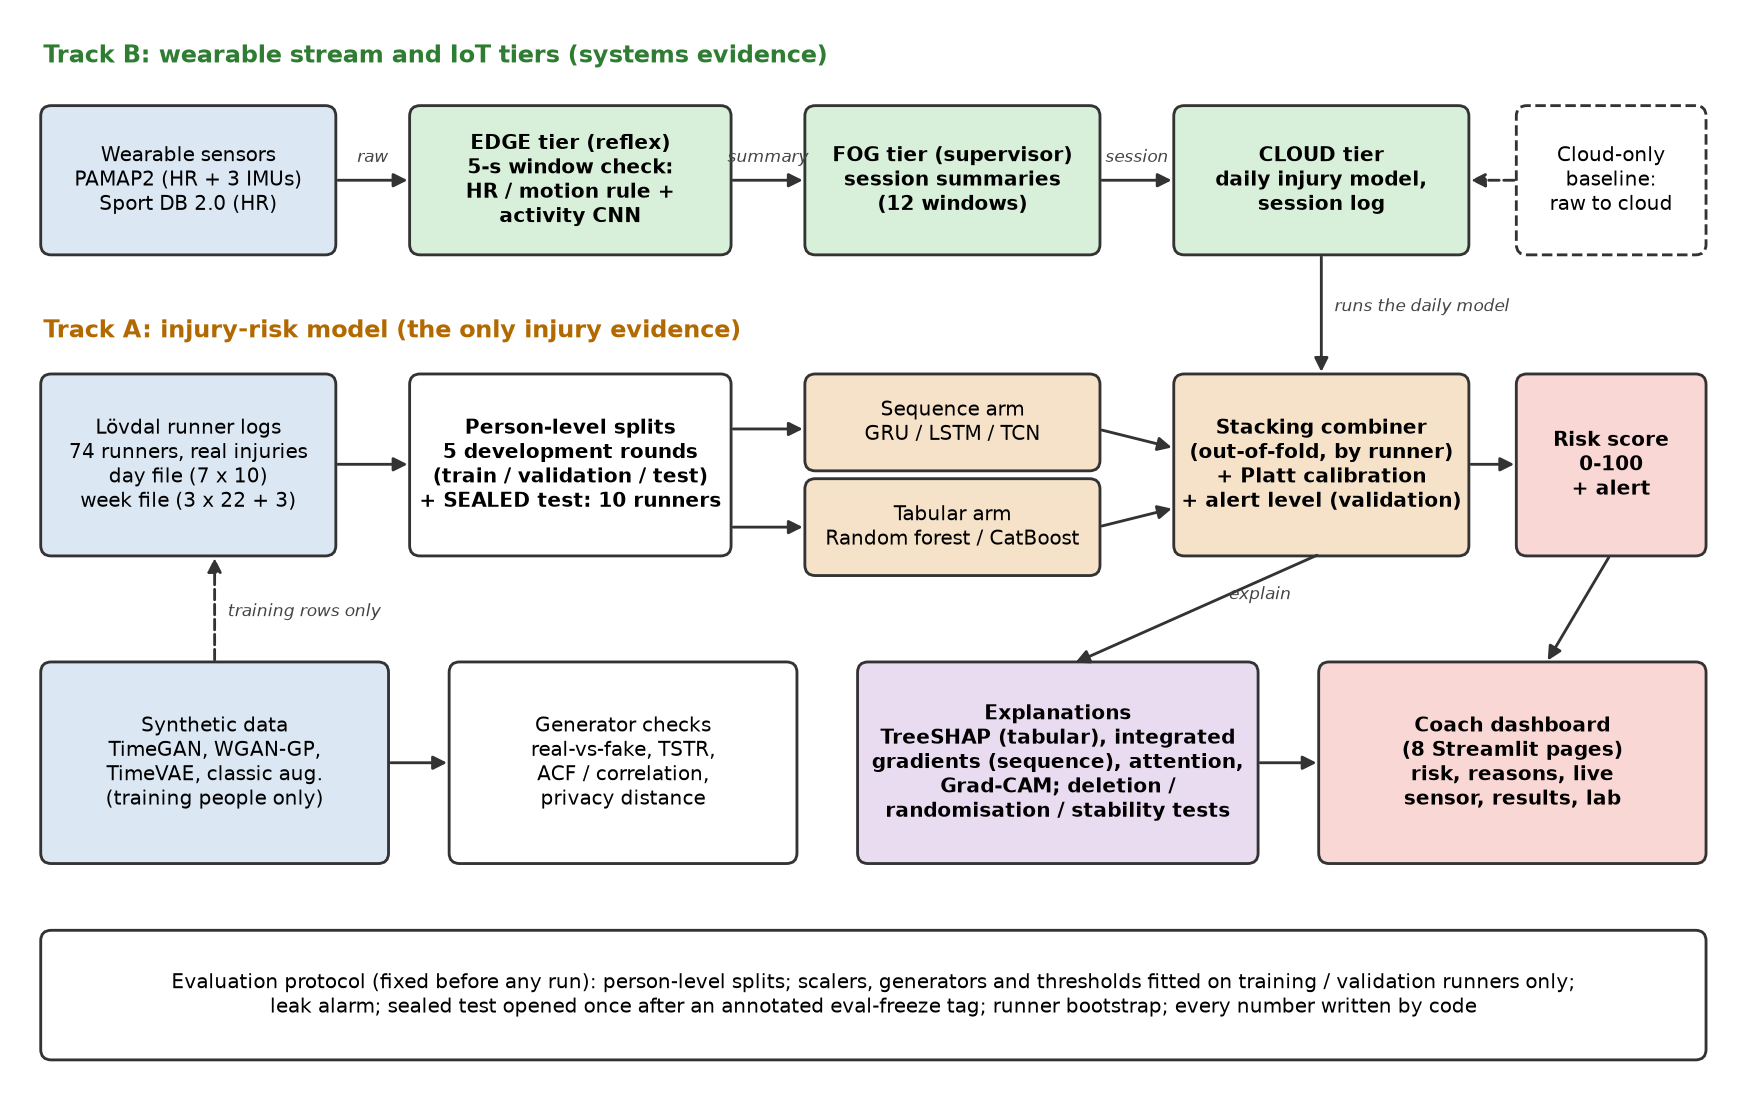
\includegraphics[width=\textwidth]{0_architecture.png}
\caption{Architecture of SynAthlete-AIoT. Track B carries the wearable stream through the edge,
fog and cloud tiers; Track A turns real runner logs into a calibrated 0--100 injury-risk score.
Synthetic data enter training rows only, and the sealed test runners are opened once.}
\label{fig:arch}
\end{figure}

\subsection{Evaluation protocol}
\textbf{Splits.} All splits are by person. The ten most recently joined runners form a sealed
final test. The other 64 runners form five development rounds; in each round, settings, early
stopping, calibration and the alert level use that round's validation runners only, and its
test runners are scored once. The sealed runners can be loaded only through a guarded function
that checks an annotated, pushed \texttt{eval-freeze} tag and an unchanged code tree, and it
records every opening.

\textbf{Leakage controls.} One z-score scaler is fitted on training runners only. Identity,
date and own-history inputs are excluded, because a runner's own event history reveals the label
in this dataset. A shuffled-label model acts as a leak alarm; its ROC-AUC stayed at
\canaryAuc{}, i.e.\ at chance. Independent code reviews were run before the freeze and before
reporting.

\textbf{Metrics.} For a test set with injured events $P$ and healthy events $N$, ROC-AUC is the
probability that a random injured event receives a higher score than a random healthy one,
\begin{equation}
\mathrm{AUC} = \frac{1}{|P|\,|N|}\sum_{i\in P}\sum_{j\in N}\mathbb{1}[s_i > s_j],
\end{equation}
and PR-AUC is the average precision over recall levels, whose chance level equals the injury
rate. PR-AUC is the headline metric because injuries are rare \citep{he2009}. Calibrated
probabilities are obtained by Platt scaling fitted on validation runners,
\begin{equation}
\hat p = \frac{1}{1 + \exp\!\big(-(a\,\mathrm{logit}(s) + b)\big)},
\end{equation}
and the risk score shown to the coach is the percentile of $\hat p$ among the round's validation
events. The alert level minimises $|\mathrm{sensitivity}-\mathrm{specificity}|$ on validation
runners.

\textbf{Uncertainty and comparisons.} Intervals come from a runner-level bootstrap with 2,000
resamples, resampling whole runners within each test group. Models are compared in pre-declared
pairs on the same rows; a difference counts only when its 95\% interval excludes zero. The
intervals are not adjusted for multiple comparisons, which we state wherever they are used.

\subsection{Injury models}
The baselines are constant risk, an acute-to-chronic style rule, logistic regression, random
forest, CatBoost and a gated recurrent unit (GRU) network. The L\"ovdal method was rebuilt twice:
as an exact copy, including its normalisation step that reads the labels, which was run once as a
sanity check on stand-in runners; and as a label-free variant compared on all five rounds. Each
tunable model tries eight settings per round, drawn by a seeded random search from grids written
before the first run; the chosen setting is refitted with three seeds.

The \textbf{fused model} combines a sequence arm (GRU, LSTM or temporal convolutional network)
on day sequences with a tabular arm (random forest or CatBoost) on week features. Both arms are
chosen on validation runners. Their predictions are combined by a logistic-regression stacker
trained on out-of-fold predictions grouped by runner, so the combiner never sees a prediction
made by a model that trained on the same runner. With 44 tries per round, the fused model has
the same tuning budget per component as every baseline, and it was declared in advance as the
model for the sealed test.

\subsection{Synthetic data generators}
Class-conditional TimeGAN, WGAN-GP and TimeVAE are trained only on each round's training
people; settings are chosen by validation train-on-synthetic, test-on-real (TSTR) macro-F1, except
WGAN-GP, which uses one declared setting and is reported as untuned. Classic augmentation
(jitter, scaling and time-warping) is the baseline. Four criteria were fixed in advance: a
real-versus-synthetic classifier should be close to 50\% accuracy (within 0.15), TSTR macro-F1
should be within 0.15 of real-data training, the autocorrelation and cross-channel correlation
errors should be below 0.10, and at most 5\% of synthetic windows may lie closer to a real
training window than real test windows usually do (a privacy check). For injury augmentation, a
conditional TimeGAN adds synthetic injury sequences to training rows only; validation and test
data stay real.

\subsection{Edge, fog and cloud tiers}
The three tiers run as separate processes connected by queues. All processes finish their
set-up before the first window, and windows are released at a steady pace of one every 0.1~s, so
that the measured latency is decision time rather than start-up waiting. We record the bytes that
reach the cloud and the median decision latency, for a PAMAP2 test person and a Sport DB 2.0
heart-rate recording, in tiered and cloud-only mode, with three repetitions each.

\subsection{Explanations}
TreeSHAP explains the tabular arm and integrated gradients explain the sequence arm. An
explanation-only attention model is always shown next to integrated gradients, never alone, and
one-dimensional Grad-CAM explains the activity network. Three tests with thresholds fixed in
advance check faithfulness: deletion (removing the top inputs must lower the risk at least 1.5
times more than removing random inputs), model randomisation (explanations of a model with random
weights must differ, rank correlation below 0.5) and stability (near-identical inputs must give
near-identical explanations, rank correlation above 0.8). Before running, we also wrote down
which inputs we expected to raise risk: recent load spikes, monotony and low recovery. Each risk
score is turned into a plain-language reason for the coach.

\section{Results}\label{sec:results}
\subsection{Injury prediction}
Table~\ref{tab:injury} and Fig.~\ref{fig:injury} report every injury model on runners never seen
in training. The leak alarm stayed at chance. Learned models reach ROC-AUC \injuryAucRange{},
clearly above chance but far from reliable prediction. The fused model reaches ROC-AUC
\fusedAuc{} and PR-AUC \fusedPrAuc{}. The exact copy of the published method passed its
pre-registered sanity check (day-file ROC-AUC \reproDayAuc{}), and the label-free variant
reaches ROC-AUC \labelFreeAuc{}. Because the two were scored on different runners, the effect of
the label-reading step was not measured head-to-head.
\begin{table}[t]\centering\caption{Injury prediction, mean $\pm$ SD over five development rounds (chance PR-AUC $\approx$ injury rate)}\label{tab:injury}
\footnotesize\begin{tabular}{llcc}\toprule
Model & File & PR-AUC & ROC-AUC \\\midrule
Constant risk & day & 0.013 $\pm$ 0.000 & 0.500 $\pm$ 0.000 \\
Constant risk & week & 0.013 $\pm$ 0.000 & 0.500 $\pm$ 0.000 \\
ACWR-style rule & week & 0.015 $\pm$ 0.001 & 0.540 $\pm$ 0.021 \\
Logistic regression & day & 0.022 $\pm$ 0.004 & 0.626 $\pm$ 0.019 \\
Logistic regression & week & 0.020 $\pm$ 0.004 & 0.621 $\pm$ 0.029 \\
Random forest & day & 0.019 $\pm$ 0.002 & 0.603 $\pm$ 0.024 \\
Random forest & week & 0.022 $\pm$ 0.007 & 0.614 $\pm$ 0.042 \\
CatBoost & day & 0.021 $\pm$ 0.004 & 0.598 $\pm$ 0.043 \\
CatBoost & week & 0.019 $\pm$ 0.002 & 0.606 $\pm$ 0.028 \\
GRU & day & 0.023 $\pm$ 0.006 & 0.631 $\pm$ 0.009 \\
L\"ovdal, label-free & day & 0.017 $\pm$ 0.003 & 0.584 $\pm$ 0.044 \\
L\"ovdal, label-free & week & 0.021 $\pm$ 0.006 & 0.589 $\pm$ 0.066 \\
\textbf{Fused} & shared & 0.022 $\pm$ 0.003 & 0.609 $\pm$ 0.024 \\
\bottomrule\end{tabular}\end{table}


\begin{figure}[htbp]
\centering
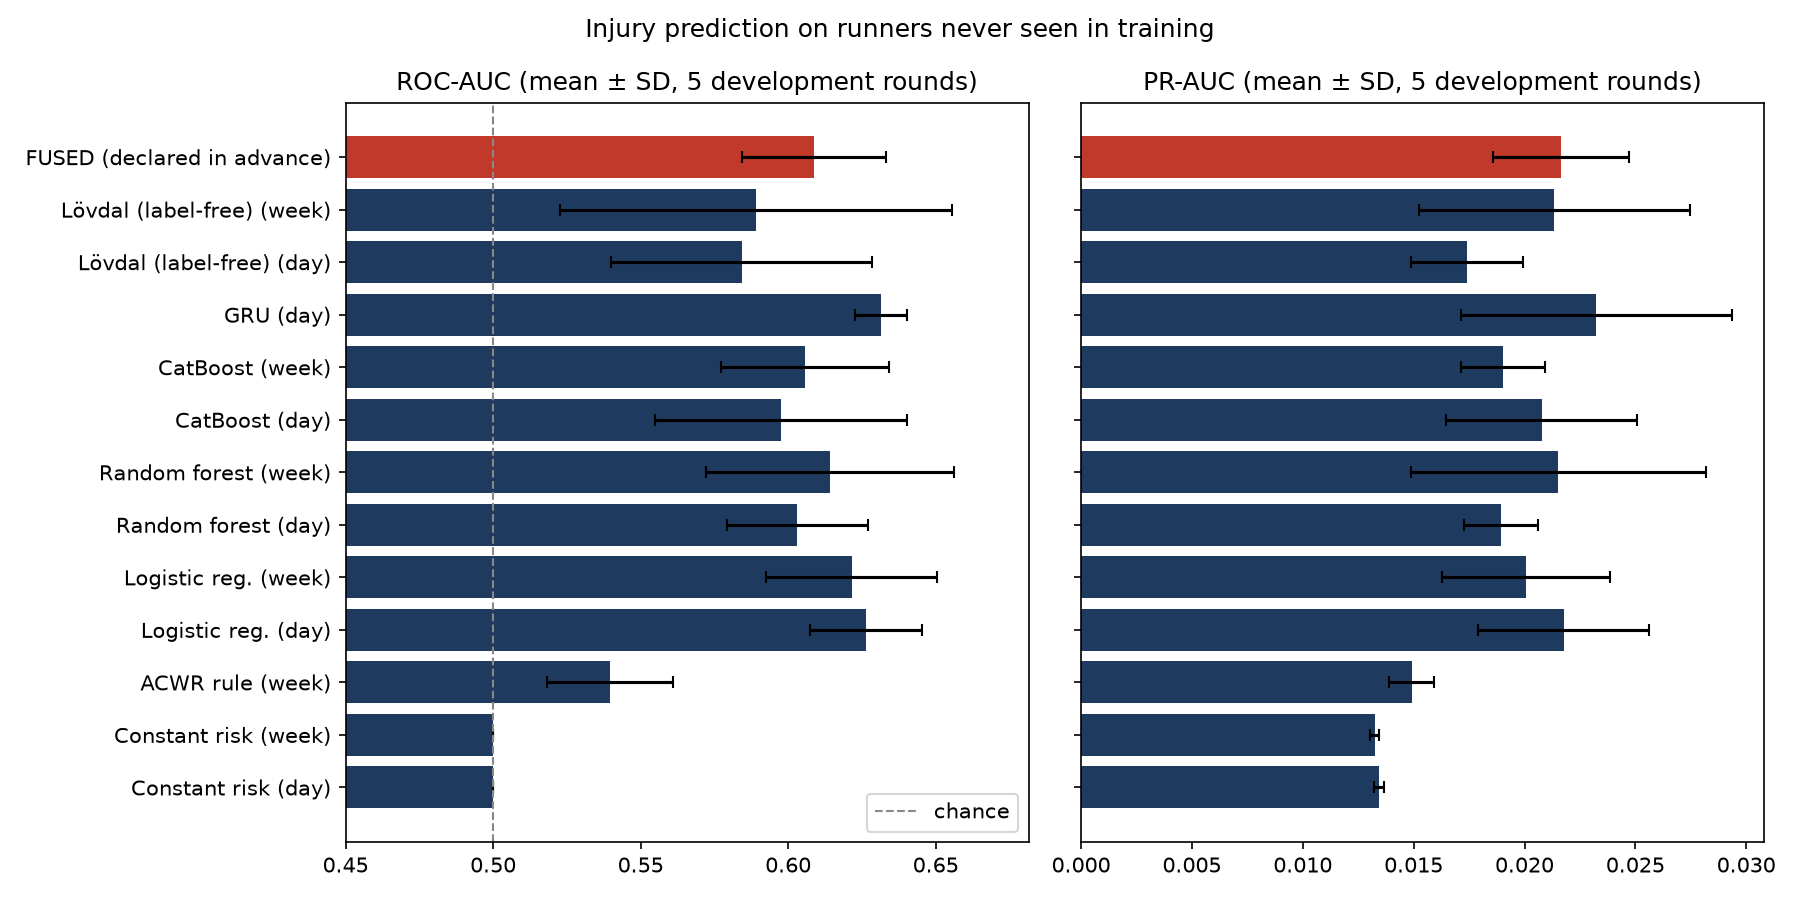
\includegraphics[width=\textwidth]{1_injury_models.png}
\caption{ROC-AUC (left) and PR-AUC (right) of every injury model, mean and standard deviation
over five development rounds. The fused model is highlighted because it was declared in advance,
not because it was best.}
\label{fig:injury}
\end{figure}

Fig.~\ref{fig:confusion} shows what an alert means in practice. At the alert level chosen on
validation runners, the fused model catches a majority of injuries, but it also raises many false
alarms, because injured and healthy days receive overlapping scores. As an early-warning tool, it
is therefore a prompt for a conversation with the athlete rather than a diagnosis.

\begin{figure}[htbp]
\centering
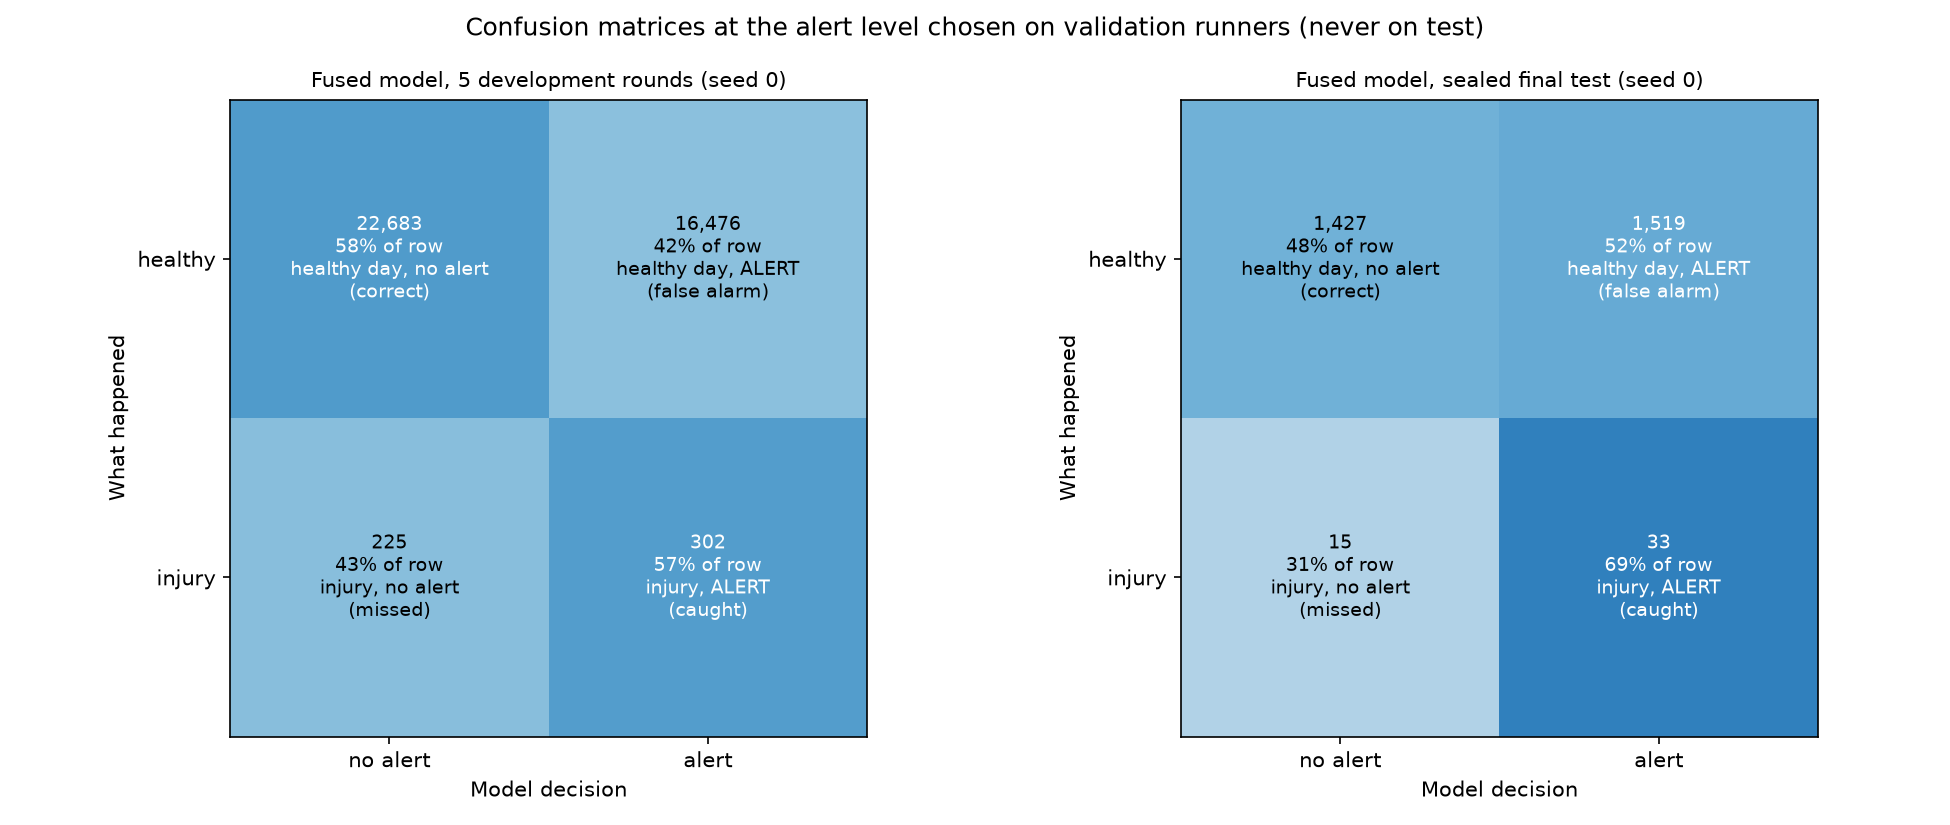
\includegraphics[width=\textwidth]{9_confusion_injury.png}
\caption{Confusion matrices of the fused model at the alert level chosen on validation runners:
pooled test runners of the five development rounds (left) and the sealed final test (right).}
\label{fig:confusion}
\end{figure}

\subsection{Sealed final test}
\lockboxSummary{} Fig.~\ref{fig:locked} places this result next to the development estimate.
The two agree, which indicates that the development results were not inflated by tuning. The
secondary results are shown for completeness only; they were scored on different rows and with
more training runners, so they are not a ranking of models.

\begin{figure}[htbp]
\centering
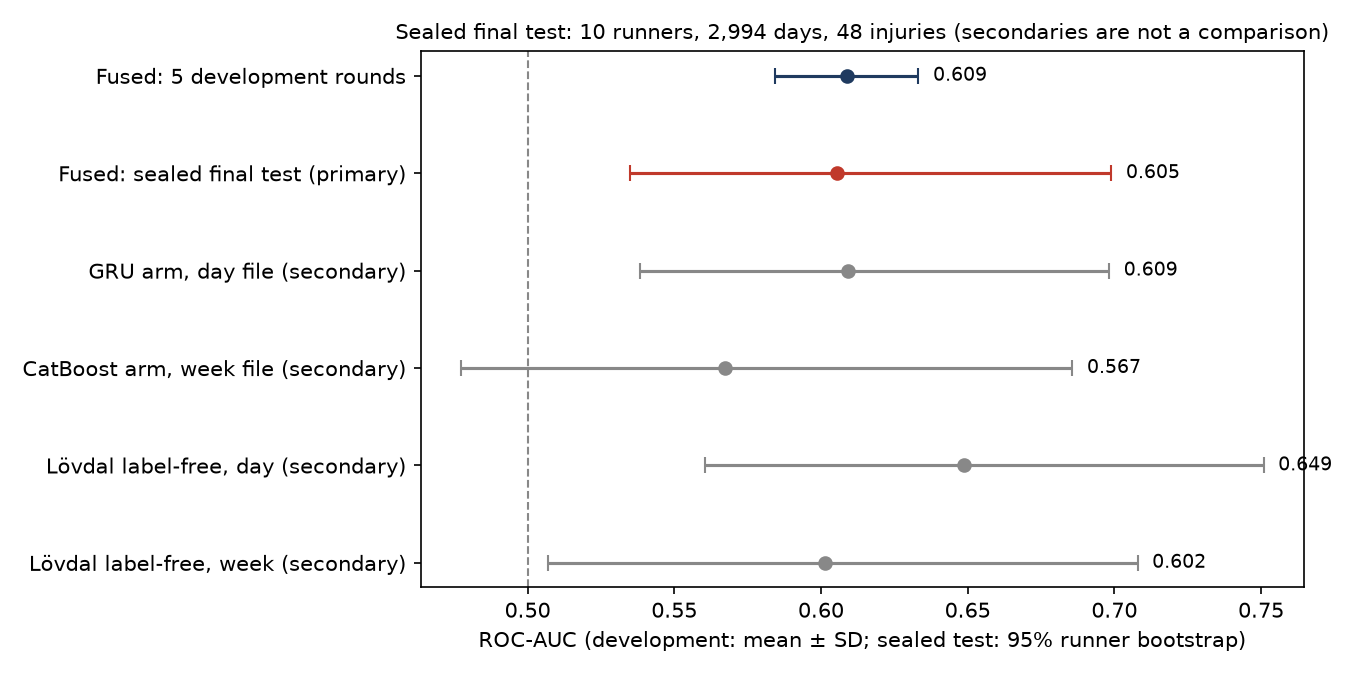
\includegraphics[width=0.92\textwidth]{2_locked_final_test.png}
\caption{Sealed final test. Development: mean $\pm$ standard deviation over five rounds; sealed
test: 95\% runner-bootstrap interval. Grey rows are secondary results and are not a
comparison.}
\label{fig:locked}
\end{figure}

\subsection{Model comparisons}
Table~\ref{tab:compare} and Fig.~\ref{fig:compare} give paired differences with runner-bootstrap
intervals. Against the label-free L\"ovdal variant, logistic regression and the GRU on the day
file are clearly better on both metrics, and CatBoost on the day file on PR-AUC only; constant
risk and the acute-to-chronic style rule are clearly worse. The fused model's gain over its
sequence arm is borderline on ROC-AUC and absent on PR-AUC, and it shows no gain over its tabular
arm. With 24 unadjusted intervals, borderline results should be read with care.
\begin{table}[t]\centering\caption{Paired differences (5-round mean, runner bootstrap 95\% interval, 2,000 resamples)}\label{tab:compare}
\footnotesize\begin{tabular}{lcc}\toprule
Comparison & $\Delta$ PR-AUC & $\Delta$ ROC-AUC \\\midrule
\multicolumn{3}{c}{n/a} \\
\bottomrule\end{tabular}\end{table}


\begin{figure}[htbp]
\centering
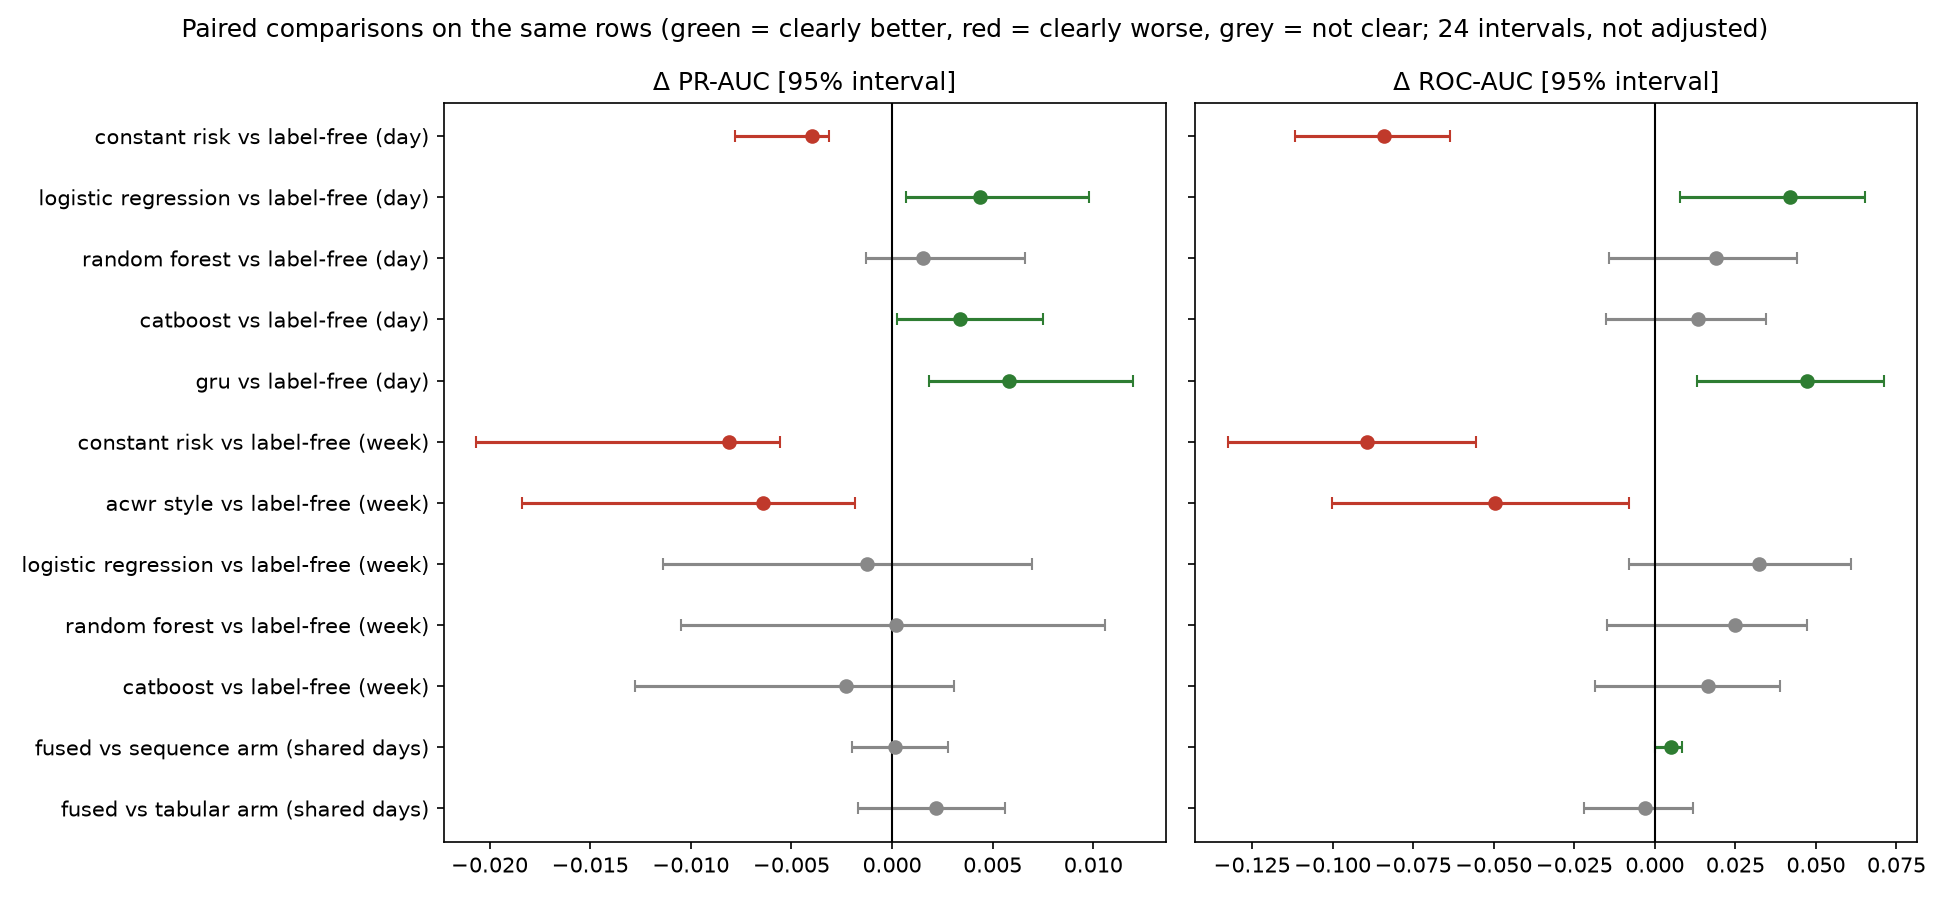
\includegraphics[width=\textwidth]{3_paired_comparisons.png}
\caption{Paired differences on the same rows with 95\% runner-bootstrap intervals (green:
clearly better; red: clearly worse; grey: not clear).}
\label{fig:compare}
\end{figure}

\subsection{Synthetic data}
Table~\ref{tab:gen} and Fig.~\ref{fig:gen} compare the generators with real-data training
(real-only macro-F1 \pamapRealFone{}). A real-versus-synthetic classifier separated the
synthetic clips of every generator easily, so no generator met the realism criterion; training on
synthetic data alone came closest to real training for classic augmentation, and adding
synthetic clips to real ones changed little. \wesadSummary{} \augmentSummary{}
\begin{table}[t]\centering\caption{Generators on PAMAP2 (4 rounds): discriminative accuracy (0.5 = indistinguishable), TSTR and real+synthetic macro-F1, pre-registered criteria passed}\label{tab:gen}
\footnotesize\begin{tabular}{lcccc}\toprule
Generator & Disc.\ acc. & TSTR & Real+syn. & Passed \\\midrule
\multicolumn{5}{c}{n/a} \\
\bottomrule\end{tabular}\end{table}


\begin{figure}[htbp]
\centering
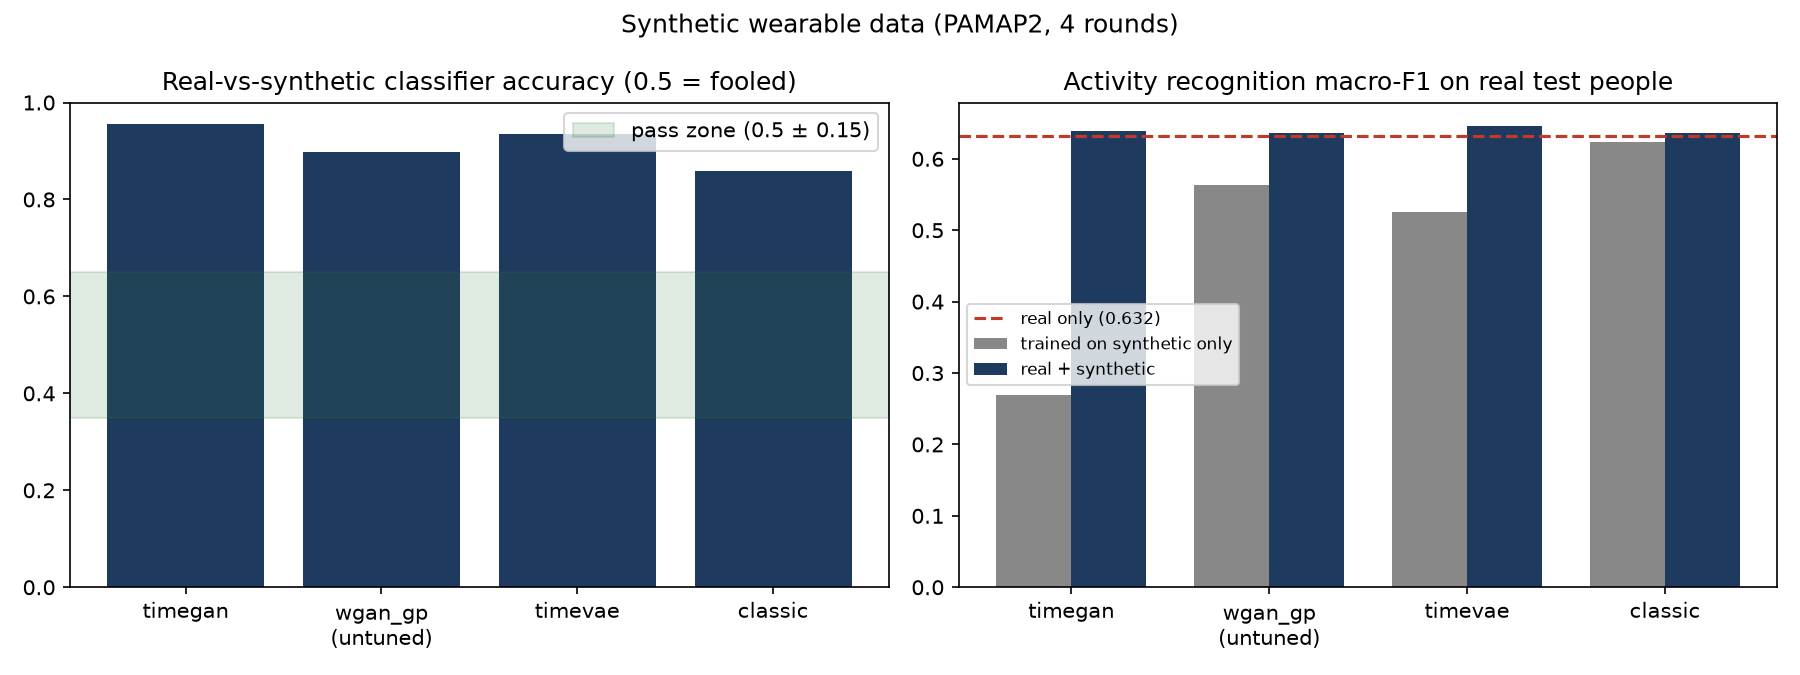
\includegraphics[width=\textwidth]{4_generators.png}
\caption{Generators on PAMAP2 (four rounds): real-versus-synthetic classifier accuracy with the
pass zone (left), and activity-recognition macro-F1 when training on synthetic data only or on
real plus synthetic data, against real-only training (right).}
\label{fig:gen}
\end{figure}

\subsection{Edge, fog and cloud tiers}
Table~\ref{tab:tiers} and Fig.~\ref{fig:tiers} show the tier benchmark. Processing at the edge
reduced the data sent to the cloud by \tiersReduction{} for the wearable stream and by
\tiersReductionHr{} for the heart-rate stream. Decisions took a few milliseconds in both modes;
because everything ran on one computer, there was no network delay to save, so latency compares
processing only and the data saving is the main result.
\begin{table}[t]\centering\caption{Edge--fog--cloud vs cloud-only (simulated on one computer)}\label{tab:tiers}
\footnotesize\begin{tabular}{llrr}\toprule
Stream & Mode & Bytes into cloud & Median decision (ms) \\\midrule
\multicolumn{4}{c}{n/a} \\
\bottomrule\end{tabular}\end{table}


\begin{figure}[htbp]
\centering
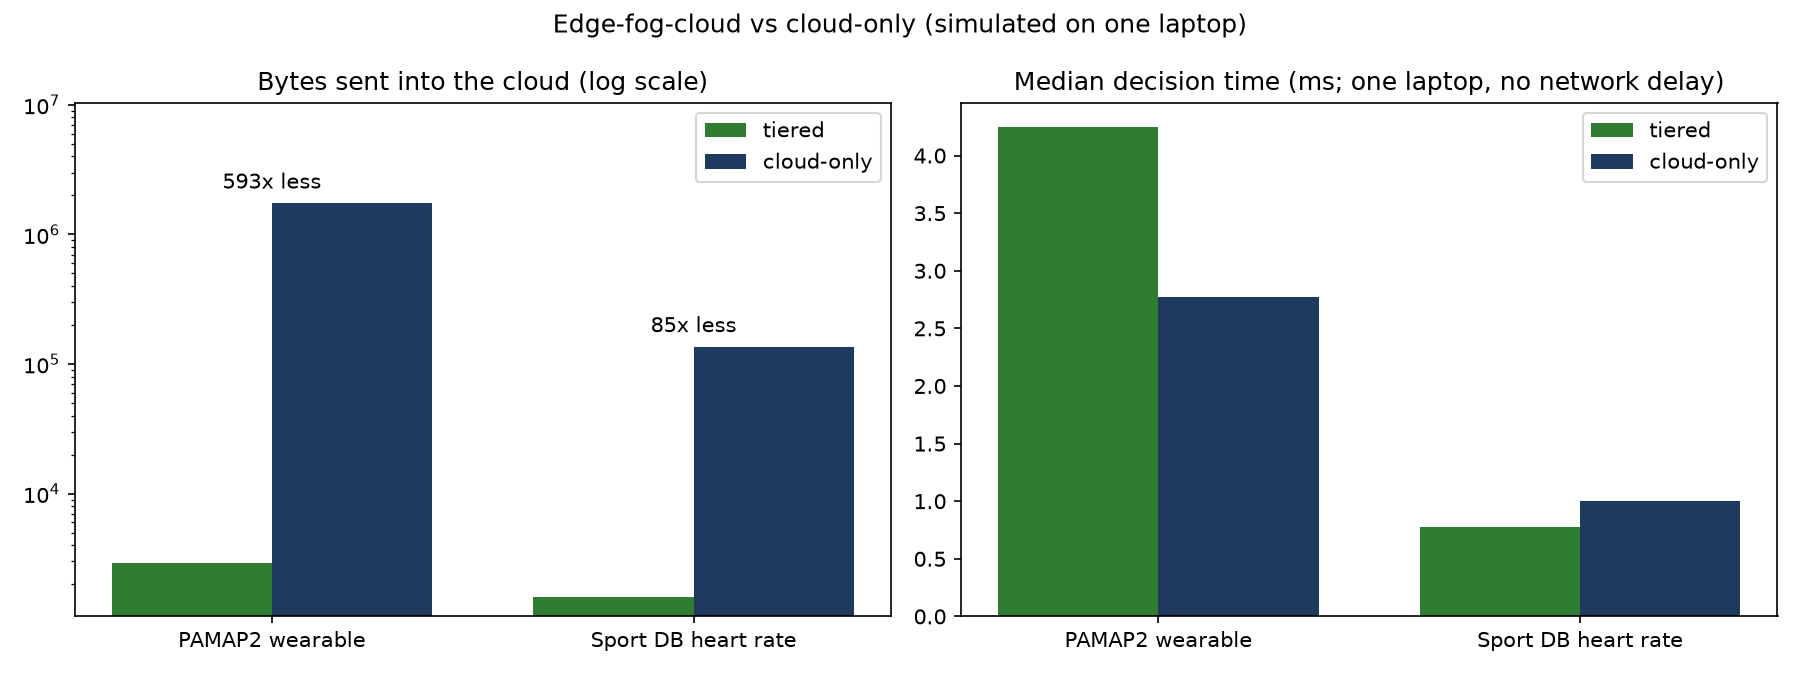
\includegraphics[width=\textwidth]{5_edge_fog_cloud.png}
\caption{Bytes sent into the cloud (left, log scale) and median decision time (right) for the
tiered design and a cloud-only design, simulated on one computer.}
\label{fig:tiers}
\end{figure}

\subsection{Explanations}
\explainSummary{} Against the expectations written before running, \explainPriors{}
(Fig.~\ref{fig:xai}). Attention weights and integrated gradients often disagreed, which supports
showing attention only next to a tested method.

\begin{figure}[htbp]
\centering
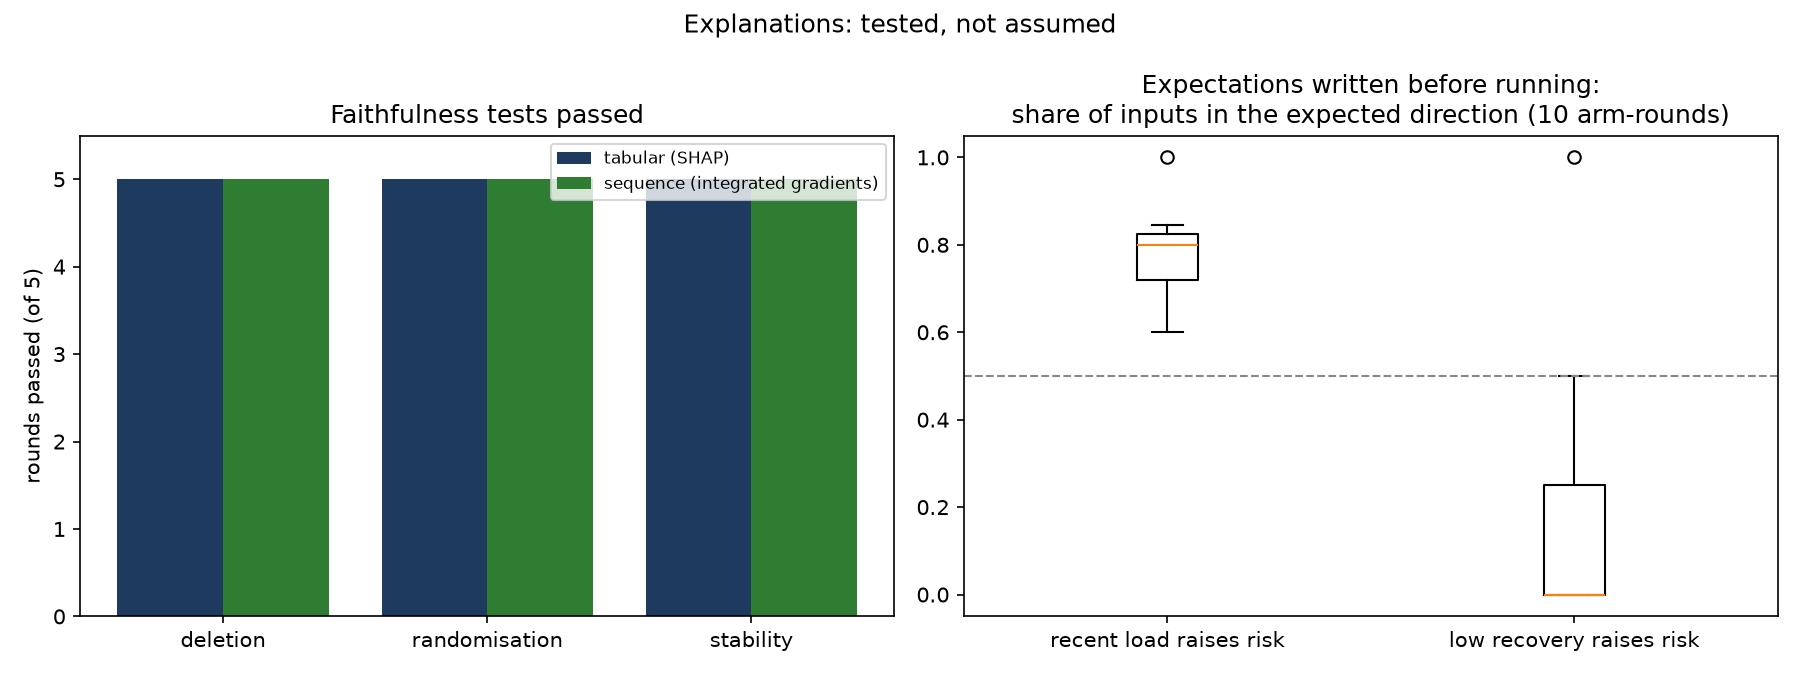
\includegraphics[width=\textwidth]{6_explanations.png}
\caption{Faithfulness tests passed per explanation method (left) and agreement with expectations
written before running (right).}
\label{fig:xai}
\end{figure}

\subsection{Discussion}
Three findings stand out. First, daily training logs carry only a weak signal before an injury:
all honest models sit modestly above chance, and the alert level that balances sensitivity and
specificity raises many false alarms. Second, the evaluation design matters: the sealed test
reproduced the development estimate, and paired intervals showed that most apparent differences
between models are not reliable. Third, the IoT design delivers a clear, measurable benefit in
data volume even though the injury signal is weak. The main limitations are the small sealed test
(ten runners), the removal of healthy days close to injuries by the dataset's authors (so alert
rates are not daily rates), the simulation of the tiers on one computer, and the fact that the
wearable participants are different people from the runners.

\section{Conclusion and Future Scope}\label{sec:conclusion}
We built and honestly evaluated a complete explainable AIoT pipeline for athlete injury risk.
Under a person-level protocol with a sealed final test, injury risk from daily training logs is
predictable only modestly, the result held on runners nobody had looked at, the edge tier sharply
reduced cloud traffic, and the explanations passed faithfulness tests. Synthetic wearable data
did not reach realism and did not improve injury prediction, which we report as a negative
result rather than hide.

Future work has five directions. (i) Collect a dataset that pairs wearable signals with real
injuries from the same athletes, so that physiology can be used as injury evidence. (ii) Deploy
the tiers on real devices and networks to measure energy use and network latency. (iii) Validate
the model prospectively on new athletes and new seasons, with larger cohorts. (iv) Improve the
generators, for example with privacy-aware training and evaluation on larger datasets. (v) Study
with coaches how risk scores and reason sentences change training decisions.

\section*{Acknowledgement}
We thank our guide and the Department for their support. AI coding assistants helped write code
and text under the authors' direction; every AI contribution is logged in the project's AI log,
every number is produced by code from saved result files, and all claims were checked by the
authors.

\bibliographystyle{elsarticle-num}
\bibliography{refs_final}

\end{document}
